
\chapter{Introdução}
\label{introducao}

Desde os primeiros sistemas comerciais estabelecidos até a Revolução Industrial,
a maneira de se fazer negócios evoluiu drasticamente. Entretanto, nada se
compara à revolução gerada com o advento da computação: a informatização das
organizações não somente permitiu-nos coletar e armazenar volumes dados
gigantescos, mas também combiná-los e processá-los com agilidade e precisão antes nunca
vistos. Com isso, geramos uma quantidade de informação humanamente impossível de
ser manipulada, o que, por sua vez, demandou desenvolver-se ferramentas e
métodos de filtragem e classificação de dados. De tal modo que minerando esses dados pode-se gerar
informação relevante a uma organização, elemento hoje imprescindível no sucesso
das decisões estratégicas de qualquer empreendimento: avaliar se uma empresa
deve pensar em expandir seu negócio (criar franquias, por exemplo) é um projeto
arriscado - se mal planejado, pode levar uma organização a sofrer sérios
prejuízos. Segundo \citeonline{Mangini2014}, a tomada de decisão em termos de
localização não pode ser feita de maneira aleatória e subjetiva, mas embasada em
um método ou ferramenta que permita determinar o melhor ponto ou o mais
adequado, de acordo com premissas objetivas e dentro de um arcabouço lógico,
considerando as possíveis variáveis que afetam aspectos relacionados ao usuário,
urbanismo e também relacionado à gestão e às políticas públicas. Neste contexto
de união entre o marketing com noções de geografia e análise de vantagens
locacionais, o \emph{geomarketing} surge como tendência para a determinação de
pontos específicos para a criação ou ampliação de uma empresa, mas que também pode ser aplicado em âmbito público.

Em vista do previamente exposto, este trabalho optou por embasar-se em
ferramentas e técnicas de análise de \emph{geomarketing} aliadas às redes de
Internet sem fios e dispositivos móveis para desenvolver
um sistema que mede o tráfego de pessoas em determinadas zonas e identifica o
perfil desses indivíduos quanto ao aparelho móvel que utilizam.

\section{Justificativa}
\label{justificativa}

A escolha da tecnologia mobile como forma de contagem se justifica pelo fato de que, hoje, a grande maioria das pessoas tem um aparelho celular. A \autoref{dados2017} mostra tabela calculada a partir de dados disponibilizados pela Anatel por \citeonline{Teleco} - ainda, segundo mesma fonte, o Brasil terminou Março de 2017 com 242,8 milhões de celulares e densidade de 117,20 cel/100 habitantes. Estimativas do \citeonline{IBGE2017} apontam para 2017 uma população de aproximadamente 207.500.000 brasileiros, mostrando que é possível considerar que cada brasileiro tem pelo menos 1 celular smarthphone - esses aparelhos, munidos de rede wi-fi, serão considerados neste trabalho - a rede sem fio será necessária no levantamento de dados. A escolha também será adequada ao tipo de tecnologia a ser empregada no dispositivo hardware em que o software será implementado, devido à compatibilidade e especificações. Sendo ainda um método de baixo custo, oferece ao cliente final um custo-beneficio mais atrativo, tornando o produto mais acessível.

\begin{figure}[htb]
  \caption{\label{dados2017}Quantidade de Celulares no Brasil - Março 2017}
  \begin{center}
    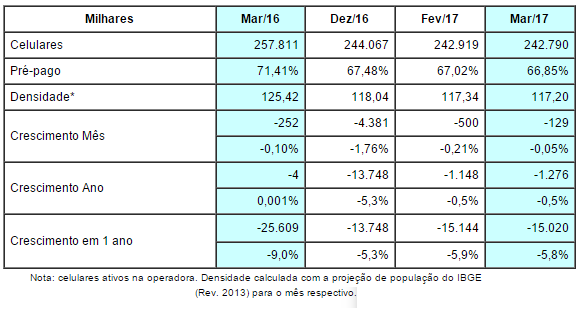
\includegraphics[width=1.0\textwidth]{img/dados2017.png}
  \end{center}
  \legend{Fonte: \citeonline{Teleco}.}
\end{figure}


\section{Objetivos}
\label{objetivos}

\subsection{Objetivos Gerais}
Este trabalho tem como objetivo desenvolver um sistema que determina o tráfego de pessoas em áreas através da comunicação
entre dispositivos móveis e redes Wi-Fi, bem como identificar o perfil desses usuários quanto ao dispositivo que utilizam.

\subsection{Objetivos específicos}
\begin{itemize}
  \item Definir os motivos pelos quais uma organização utiliza o \emph{geomarketing};
  \item Identificar casos de uso do tráfego de indivíduos em ambientes como técnica
  de \emph{geomarketing};
  \item Estudar ferramentas de contagem de pessoas em ambientes;
  \item Definir as tecnologias para identificação e fornecimento de dados de usuários;
  \item Identificar a tecnologia responsável pela contagem de pessoas;
  \item Definir o modo como o número de indivíduos será agrupado para gerar o tráfego;
  \item Indicar como os dados capturados serão agrupados para gerar perfis de usuário;
  \item Implementar interface para apresentar o tráfego e os perfis das pessoas identificadas;
  \item Testar o sistema em ambientes controlados e não controlados;
  \item Realizar ajustes para garantir precisão do sistema desenvolvido.
\end{itemize}

\section{Organização do trabalho}
O presente trabalho divide-se em capítulos, sendo este o primeiro (Introdução). Os demais capítulos são:

\begin{itemize}
  \item \textbf{Fundamentação Teórica:} apresentação dos conceitos teóricos envolvidos no trabalho, motivação de
  adoção de certas tecnologias para a construção do sistema e soluções semelhantes;
  \item \textbf{Metodologia:}ferramentas escolhidas para o desenvolvimento, métodos de testes, planos de contingência e módulos
  do sistema;
  \item \textbf{Cronograma:}módulos que serão entregues nos respectivos períodos indicados.
\end{itemize}
